\section{Preprocessing}
\label{sec:preprocess}
%%%%%%%%%%%%%%%%%%%%%%%%%%%%%%%%%%%%%%%%%%%%%%%%%%%%%%%%%%%%%%%%%%%%%%%%%%%%%%%%%%%%%%%%%%%%%%%%%%

This work leverages both OD trails and road network to improve edge bundling quality.
This section introduces major steps in \textit{Preprocessing} stage, including: map matching, hierarchical road structure construction, and trail abstraction.

%%%%%%%%%%%%%%%%%%%%%%%%%%%%%%%%%%%%%%%%%%%%%%%%%%%%%%%%%%%%%%%%%%%%
\subsection{Basic Traffic Concepts}
\textit{Road Network}:
A road network can be modeled as a directed graph $\bar{G} = (\bar{V}, \bar{E})$, where $\bar{V}$ is the set of nodes in $\bar{G}$ and $\bar{E}$ is the set of edges connecting nodes in $\bar{V}$.
Degree of a vertex $\bar{v}$, denoted as $deg(\bar{v})$, indicating the number of edges connected to $\bar{v}$.
By this, a vertex $\bar{v} \in \bar{V}$ can be classified as an endpoint with $deg(\bar{v})=1$, a midpoint with $deg(\bar{v})=2$, or an intersection with $deg(\bar{v})>2$.
To facilitate computation, we can simply $\bar{G}$ into a simplified graph $G = (V, R)$, where $V$ is the union of endpoints and intersections, and $R$ is a set of links connecting nodes in $V$.
Each link $r$ represents a sequence of $n$ consecutive nodes in $\bar{V}$:

\vspace{-5mm}
\begin{equation}
  \begin{aligned}
  	r &:= \bar{v}_1 \rightarrow \bar{v}_2 \rightarrow ... \rightarrow \bar{v}_n, \,\,\, \forall \bar{v}_i \in \bar{V}
  \end{aligned}
\end{equation}

\vspace{-2mm}
\noindent
where $\bar{v}_1$ and $\bar{v}_n$ are endpoints or intersections, while the other nodes are midpoints.
For the sake of clarity, we use the term \textit{route} to describe such a link.
Computation tasks, including shortest path query and map matching, are performed on the simplified graph $G$.

\vspace{1mm}
\noindent
\textit{Urban Traffic}:
Thanks to open data campaign, many urban traffic data are available nowadays.
Typically, raw urban traffic data can come in either of the following forms:

\begin{itemize}
\item
\textit{UT-1}: origin and destination locations only, such as New York taxi trips~\cite{ferreira2013visual} and Singapore public transportation rides~\cite{zeng_2015_visualizing}.
Such a raw trip $t_{raw}$ can be represented as $t_{raw} := l_o \rightarrow l_d$, where $l_o$ and $l_d$ represent origin and destination locations, respectively.

\item
\textit{UT-2}: a sequence of GPS positions, such as Stuttgart scooter fleet~\cite{kruger_trajectorylenses_2013} and Hangzhou taxi trips~\cite{wang_2014_visual-reasoning}.
Such a raw trip $t_{raw}$ can be represented as $t_{raw} := l_1 \rightarrow l_2 \rightarrow ... \rightarrow l_n$, where $l_i \subset \mathbb{R}^2$. $l_1$ and $l_n$ are origin and destination, i.e., $l_o$ and $l_d$.
\end{itemize}

Both forms of urban traffic data can be generalized as a traffic graph $G_t = (L, T)$, where $L$ is the set of locations and $T$ is the set of trips represented as sequential connections of locations.

%%%%%%%%%%%%%%%%%%%%%%%%%%%%%%%%%%%%%%%%%%%%%%%%%%%%%%%%%%%%%%%%%%%%%%%
\subsection{Map Matching}
\label{section:edge_matching}

Constraining movements over an underlying road network, i.e., mapping traffic graph $G_t := (L, T)$ to road network $G := (V, R)$, is usually a preliminary step for urban traffic analysis.
This is necessary.
First, recorded locations get errors due to imprecise GPS localization, while road network is precise and constant.
Second, $G_t$ can be much more complex than $G$:
Taking New York traffic for an example, there are over millions of taxi trips per day, resulting in millions of locations $L$, yet its simplified road network contains less than 100K routes.
Therefore, map matching can enrich effective analysis and visualization.

There are many map matching methods available, including shortest path, minimum turns, and ST-matching~\cite{lou_2009_map} for GPS traces.
These methods are preferable for different dataset.
We employ the following methods for corresponding urban traffic.

\begin{itemize}

\item
For \textit{UT-1}, i.e., $t_{raw} = l_o \rightarrow l_d$, we first find corresponding closest nodes $v_o \in V$, $v_d \in V$ for $l_o$ and $l_d$ respectively.
After that, we search for the shortest path between $v_o$ and $v_d$ in $G$.

\item
For \textit{UT-2}, i.e., $t_{raw} = l_1 \rightarrow l_2 \rightarrow ... \rightarrow l_n$, we use ST-matching algorithm, which considers not only spatial features of road network, but also temporal constraints.
The method was later visually investigated and optimized with an interactive interface~\cite{kruger_2018_visual}.
\end{itemize}

Both methods return a sequence of routes $r_1 \rightarrow r_2 \rightarrow ... \rightarrow r_n$ in $G$ for each OD trail $t_{raw}$.
We then combine the routes with origin ($l_o$) and destination ($l_d$) locations of $t_{raw}$.
Thus, both types of $t_{raw}$ are converted to the same map matching form. 

\vspace{-4mm}
\begin{equation}
  	\begin{aligned}
t_{map} := l_o \rightarrow r_1 \rightarrow r_2 \rightarrow ... \rightarrow r_n \rightarrow l_d.
 	\end{aligned}
\end{equation}
\vspace{-3mm}

Here the OD trail's origin $l_o$ and destination $l_d$ are kept.

%%%%%%%%%%%%%%%%%%%%%%%%%%%%%%%%%%%%%%%%%%%%%%%%%%%%%%%%%%%%%%%%%%%%%%%%%%%%%%%%%%%%%%%%%%%%%%%%%%
\subsection{Hierarchical Route Structure Construction}
\label{ssec:hiera_road}

\begin{table}
	\centering
	\begin{tabular}{|c|c|c|}
	\hline
	Category & Exemplary OSM Indicator & Score ($r_{hier}$)  \\ \hline
	Expressway & motorway, trunk & 1 \\ \hline
	Trunk Road & primary, motorway\_link& 0.75 \\ \hline
	Secondary Road & secondary, tertiary & 0.5 \\ \hline
	Branch Road & unclassified, residential & 0.25 \\ \hline
	\end{tabular}
	\vspace{1mm}
	\caption{Route hierarchy, OSM indicator and hierarchy score} \label{tab:sometab}
	\label{table: road_score}
\vspace{-6mm}
\end{table}

A road network is usually designed in hierarchical levels to avoid dense direct connections among regions.
This inspires us to construct a hierarchical route structure to benefit edge bundling.
Although urban roads are organized hierarchically, it does not consider OD trails.
This work makes use of the following attributes of a route $r$ in $G := (V, R)$ to construct a hierarchical route structure.

\vspace{1mm}
\noindent
\textit{Route length} ($len(r)$).
Visual appearance of each OD trail is determined by its routes on road network.
Longer a route, more it will affect the visual appearance.
Thus an important component affecting route hierarchy is route length.
Here, $len(r)$ is measured in Euclidean space and normalized over the whole road network.

\vspace{1mm}
\noindent
\textit{Road hierarchy} ($hier(r)$).
Urban roads are classified into hierarchies: freeways, arterials, collectors, and local roads.
Similar descriptions can also be found elsewhere~\cite{wang_2014_visual-reasoning}.
A higher level usually indicates faster traffic speed and less access to property.
OSM provides more detailed indicators of road hierarchy, e.g., trunk, primary, tertiary, etc.
To keep consistent, we classify these indicators into four hierarchies.
A route $r$ in each hierarchy is assigned an score according to Table~\ref{table: road_score}. 

\vspace{1mm}
\noindent
\textit{Flow magnitude} ($flow(r)$).
Flow magnitude measures how many OD trails pass through a route $r$.
The previous two factors purely rely on road network, while $flow(r)$ reflects the importance of a route in consideration of OD trails.
Here, $flow(r)$ is measured by counting how many mapped OD trails passing through $r$, and then normalized. 

\vspace{2mm}
By this, each route can be represented by a vector $V(r) := <len(r), hier(r), flow(r)>$.
Score of a route $score(r)$ can be measured as $score(r) = \sum w_i \times V(r)_i$, where the weights $w_i (i = 1, 2, 3)$ controls how much each attribute affects route weight.
We choose 0.3, 0.1, and 0.6 in this work, which highlights the importance of flow magnitude.
In the end, all routes are sorted in descending order according to their weights.
The routes $R$ are further subdivided into multiple hierarchical levels $R^1$, $R^2$, ..., $R^n$.
Each level of routes accounts for top-k routes.

\begin{figure}[t]
	\centering
	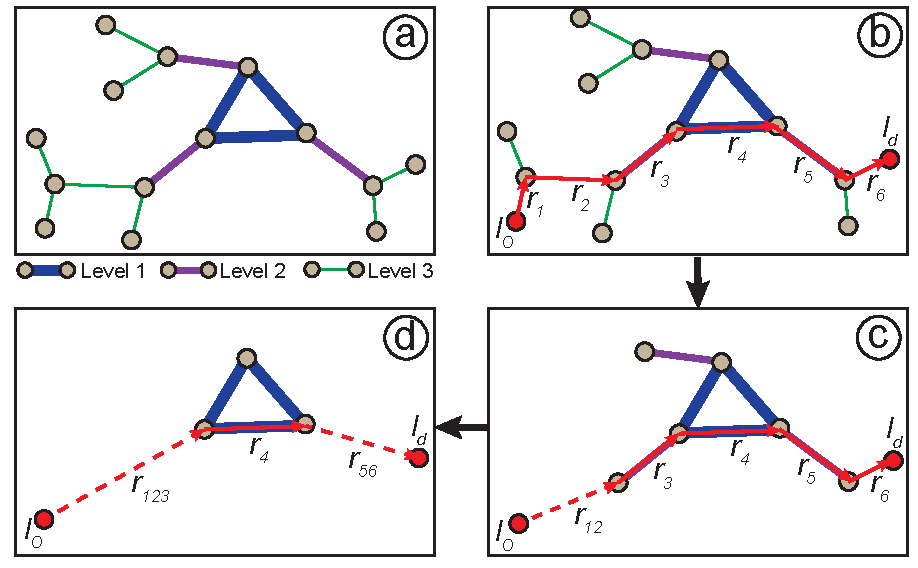
\includegraphics[width=0.45\textwidth]{figure/edgebundling/fig4_od_abstraction/OD_Abstraction.pdf}
	\vspace{-3mm}
	\caption{Illustration of hierarchical route structure and OD trail abstraction:
	(a) Three route levels are constructed colored in blue, purple and green, repsectively; a raw OD trail is abstracted in accordance to route (b) level-3, (c) level-2, and (d) level-1.}
	\label{fig:road_hierarchy}
	\vspace{-6mm}
\end{figure}

%%%%%%%%%%%%%%%%%%%%%%%%%%%%%%%%%%%%%%%%%%%%%%%%%%%%%%%%%%%%%%%%%%%%%%%%%%%%%%%%%%%%%%%%%%%%%%%%%%
\subsection{Trail Abstraction}
\label{section: trail_abstraction}

\textbf{P2} states that road network is omitted in original KDEEB, which can lead to wrong depiction in geographical space and poor support of multi-scale exploration.
We introduce a new parameter of route awareness $p_{ra}$, which defines the level of trail abstraction, to tackle this issue.
Higher $p_{ra}$ indicates that more details of OD trails should be preserved.
Given a hierarchical route structure in $n$ levels, $p_{ra}$ can range from 0 to $n$.
If $p_{ra}$ is set to zero, OD trails will be abstracted to straight lines connecting ODs directly.
If $p_{ra}$ is set to $n$, no abstraction will be applied.
If $p_{ra}$ is set to a value $m$ in [1, $n-1$], routes in level-1 to level-$m$ will be preserved.

Figure~\ref{fig:road_hierarchy}(a) presents an exemplary road network with a hierarchical route structure.
The routes are categorized into three levels: blue thick lines for level 1, purple medium lines for level 2, and green thin lines for level 3.
Figure~\ref{fig:road_hierarchy}(b-d) illustrates an example of how a raw OD trail of $l_o \rightarrow r_1 
\rightarrow...\rightarrow r_6 \rightarrow l_d$ can be abstracted in accordance to the hierarchical route structure shown in Figure~\ref{fig:road_hierarchy}(a).
In Figure~\ref{fig:road_hierarchy}(b), $p_{ra}$ is set 3, and all routes are preserved.
In Figure~\ref{fig:road_hierarchy}(c), $p_{ra}$ is set 2, so route $r_1$ and $r_2$ will be merged together as they are both level-3 routes.
In Figure~\ref{fig:road_hierarchy}(d), $p_{ra}$ is set 1, thus only route $r_4$ will be kept.